\documentclass[11pt,a4paper]{article}
\usepackage[utf8]{inputenc}
\usepackage[lmargin=2.5cm,rmargin=2cm,tmargin=3cm,bmargin=2.5cm]{geometry}
\usepackage[spanish]{babel}
\linespread{1.5}
\usepackage{graphicx}
\usepackage[dvipsnames,usenames]{color}

\title{\LARGE{\textbf{Método en diferencias Finitas para resolver la ecuación de calor en estado estacionario}}}
\date{Diciembre 4, 2015}
\author{Moreno Vera, Felipe Adrian\\ Facultad de Ciencias, Universidad Nacional de Ingeniería\\Email: felipe.moreno.v@uni.pe } %, \LaTeX\ Academy}
\begin{document}
\maketitle
\tableofcontents
\listoftables
\listoffigures
\newpage
\section{Premiliminares}
\subsection{Ecuaciones Diferenciales Parciales}
\thispagestyle{empty}
Consideremos la ecuación diferencial parcial ... (*)
$$
A\frac{\partial^2u}{\partial x^2} + 2B\frac{\partial^2u}{\partial x \partial y}+ C\frac{\partial^2u}{\partial y^2} +D\frac{\partial u}{\partial x}+E\frac{\partial u}{\partial y}= F
$$
en
$ a \le x \le b $ donde: \[u(a) = u_{\alpha} ~~ y ~~ u(b) = u_{\beta}\] 

Con condiciones de frontera Dirichlet ( en este caso ) u otro tipo de frontera. Para usar el procedimiento general de solución numérica mediante el método de diferencias finitas, debemos hacer:\\
\newline
1. Generar una malla del dominio, una malla es un conjunto finito de puntos en los cuales buscaremos la solución aproximada a la ecuación diferencial parcial.
\\
2. Sustituir las derivadas correspondientes con algunas de las f[ormulas de diferencias finitas centradas, en cada punto donde la solución es desconocida para obtener un sistema algebraico de ecuaciones Au=f.\\
3. Resolver el sistema de ecuacién es y asi obtener la solución aproximada en cada punto de la malla.
\newline
Se tiene la ecuación *, de donde se construye una matriz con los coeficientes A,B y C.

$$
Z=\left\{\begin{array}{crl}
    A & B\\
    B & C
    \end{array}\right\}
$$

En función del determinante la ecuación (*):\\
1. Se dice elíptica si la matriz Z tiene un determinante mayor a 0.\\
2. Se dice parabólica si la matriz Z tiene un determinante igual a 0.\\
3. Se dice hiperbólica si la matriz Z tiene un determinante menor a 0.\\
\\
Aparte se presentan los tipos conocidos de ecuaciones parciales que son mas frecuentes como se ve en la tabla~\ref{tabla1}

\begin{table}[htb]
\begin{center}
\begin{tabular}{|l|l|l|}
\hline
Ecuación & Nombre & Tipo \\
\hline \hline \hline
$\nabla^2 u=0$ & Laplace & Elíptica \\ \hline
$\frac{\partial^2u}{\partial t^2}=c^2 \nabla^2 u$ & Onda & Hiperbólica \\ \hline
$\frac{\partial u}{\partial t}=k \nabla^2 u$ & Difusión & Parabólica \\ \hline
$\nabla^2 u=ku$ & Helmholtz & Elíptica \\ \hline
\end{tabular}
\caption{Tipos de ecuaciones diferenciales parciales de orden 2.}
\label{tabla1}
\end{center}
\end{table}

\newpage
\subsection{Método de Diferencias Finitas en 2 Dimensiones}
\thispagestyle{empty}
Con las condiciones iniciales que nos brindan para el dominio de $ a \le x \le b $ y $ c\le y \le d$ donde se crea una malla de puntos de la forma mostrada en la figura ~\ref{figura1}\\
\begin{figure}[htbp]
\begin{center}
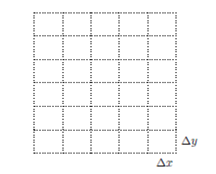
\includegraphics[scale=1.25]{img_1}
\caption{Malla en el dominio}
\label{figura1}
\end{center}
\end{figure}
\\
Donde los puntos que estan en el borde de los $\triangle x$ y $\triangle y$ son los puntos de frontera de dicha ecuación.
Luego los puntos interiores, son nuestras incognitas a encontrar, mientras mas diviones halla, mas variables tendremos que resovler y nuestro sistema de ecuaciones será de mayor dimension, es decir, si divimos el mallado en N sub intervalos por x y y, nuestro sistema será de dimension (N+1)x(N+1), donde dichas variables serán las solución es del sistema Au=f.\\
Pasamos a reemplazar por medio de diferenciación numérica por método de las Derivadas de Taylor.\\
Se debe indicar el factor de paso ( el tamaño por cada punto, es decir, la longuitud del intervalo ) h (en X) y k (en Y).\\
Construyendo el vector f mediante el siguiente algoritmo:\\

\textbf{Algoritmo 1}\\
.~~reemplazar en la ecuación direfencial parcial las aproximaciones mediante series de taylor.\\
.~~para i = 1 hasta n, hacer\\
.~~~~para j = 1 hasta n, hacer\\
.~~~~~~reemplazar y calcular los valores de frontera, y junto a las incognitas formar la matriz A y el vector u.\\
.~~~~fin para\\
.~~fin para\\
\\
Después de aplicar este algoritmo obtenemos la forma Au = f, que puede ser resuelta por cualquier método computacional de resolución de sistemas lineales de ecuaciones.\\\\
Construyendo la matriz A:\\
Los elementos de A, serán generalmente formados por los coeficientes de las aproximaciones numéricas de las derivadas entre el factor de paso.\\
\\
Construyendo el vector f:\\
Está constituido de los puntos de frontera de las ecuaciones, multiplicados por su coeficientes dados en la aproximación de la derivada, dividida entre el factor de paso.
Se obtendra una matriz simetrica que graficamente se verá asi:
$$
A=\left\{\begin{array}{cccccccc}
    A & B & M & N & ... & \alpha_1 & \beta_1 & \theta_1\\
    B & C & D & T & ... & \alpha_2 & \beta_2 & \theta_2\\
    M & D & E & F & ... & \alpha_3 & \beta_3 & \theta_3\\
    N & T & F & G & ... & \alpha_4 & \beta_4 & \theta_4\\
    . &   &   &   & ... &   &   &  \\
    \alpha_1 & \alpha_2 & \alpha_3 & \alpha_4 & ... & X & U & \theta_n\\
    \beta_1 & \beta_2 & \beta_3 & \beta_4 & ... & U & Y & W\\
    \theta_1 & \theta_2 & \theta_3 & \theta_4 & ... & \theta_n & W & Z\\
    \end{array}\right\}
$$

\section{Introduccion al problema}
\subsection{Problemática a resolver}
\thispagestyle{empty}
\subsubsection{Equilibrio Térmico}
\thispagestyle{empty}
El equilibrio térmico es aquel estado en el cual se igualan las temperaturas de dos cuerpos, las cuales, en sus condiciones iniciales presentaban diferentes temperaturas. Una vez que las temperaturas se equiparan se suspende el flujo de calor, llegando ambos cuerpos al mencionado equilibrio térmico.
\\1.Dos sistemas se dicen que están en equilibrio térmico cuando el valor de sus temperaturas es la misma.
\\2.Dos sistemas se dicen que están en equilibrio mecánico cuando el valor de sus presiones es la misma.
\\3.Dos sistemas se dicen que están en equilibrio de fases cuando el valor de sus potenciales químicos es el mismo en cada fase en que se encuentre presente la especie.
Todas las fuerzas están balanceadas.
\subsubsection{Transferencia de Calor}
El calor se define como la transferencia de energía térmica que se da entre diferentes cuerpos o diferentes zonas de un mismo cuerpo que se encuentran a distintas temperaturas, sin embargo en termodinámica generalmente el término calor significa transferencia de energía. Este flujo de energía siempre ocurre desde el cuerpo de mayor temperatura hacia el cuerpo de menor temperatura, ocurriendo la transferencia hasta que ambos cuerpos se encuentren en equilibrio térmico (ejemplo: una bebida fría dejada en una habitación se entibia).
\\
El calor puede ser transmitido de tres formas distintas: por conducción, por convección o por radiación.
\\
1. Conducción térmica: es el proceso que se produce por contacto térmico entre dos ó más cuerpos, debido al contacto directo entre las partículas individuales de los cuerpos que están a diferentes temperaturas, lo que produce que las partículas lleguen al equilibrio térmico. Ej: cuchara metálica en la taza de té.\\
\\
2.Convección térmica: sólo se produce en fluidos (líquidos o gases), ya que implica movimiento de volúmenes de fluido de regiones que están a una temperatura, a regiones que están a otra temperatura. El transporte de calor está inseparablemente ligado al movimiento del propio medio. Ej.: los calefactores dentro de la casa.\\
\\
3.Radiación térmica: es el proceso por el cual se transmite a través de ondas electromagnéticas. Implica doble transformación de la energía para llegar al cuerpo al que se va a propagar: primero de energía térmica a radiante y luego viceversa. Ej.: La energía solar.
\\
\\La conducción pura se presenta sólo en materiales sólidos.\\La convección siempre está acompañada de la conducción, debido al contacto directo entre partículas de distinta temperatura en un líquido o gas en movimiento.\\En el caso de la conducción, la temperatura de calentamiento depende del tipo de material, de la sección del cuerpo y del largo del cuerpo. Esto explica por qué algunos cuerpos se calientan más rápido que otros a pesar de tener exactamente la misma forma, y que se les entregue la misma cantidad de calor.\\Nosotros nos centraremos en la Conducción térmica. ver figura ~\ref{figura2}
\begin{figure}[htbp]
\begin{center}
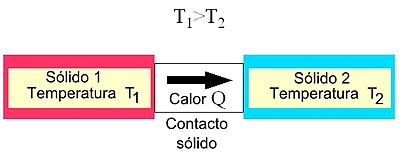
\includegraphics[scale=1.25]{img_2}
\caption{Conduccion Termica}
\label{figura2}
\end{center}
\end{figure}


\subsection{Planteamiento del Problema}
\thispagestyle{empty}
Para saber como cambia la Temperatura(variable clave) con respecto al tiempo se formula la ecuación de Calor, la ecuación del calor es una importante ecuación diferencial en derivadas parciales parabólica que describe la distribución del calor (o variaciones de la temperatura) en una región a lo largo del transcurso del tiempo. Para el caso de una función de 2 variables en el espacio (x,y) y la variable temporal t, la ecuación del calor es:
$$
\frac{\partial^2 T}{\partial x^2} + \frac{\partial^2 T}{\partial y^2} = \frac{1}{\alpha} \frac{\partial T}{\partial t} ....(1)
$$
Donde reemplazando en la ecuación general de la forma: $
A\frac{\partial^2u}{\partial x^2} + 2B\frac{\partial^2u}{\partial x \partial y}+ C\frac{\partial^2u}{\partial y^2} +D\frac{\partial u}{\partial x}+E\frac{\partial u}{\partial y}= F
$, se obtiene A=C=1, B=D=E=0, entonces la matriz Z definida por:
$
Z=\left\{\begin{array}{crl}
    A & B\\
    B & C
    \end{array}\right\}
$
\\Será igual a $
Z=\left\{\begin{array}{crl}
    1 & 0\\
    0 & 1
    \end{array}\right\}
$, con Determinante $\mid Z\mid$=$1 \gg 0 $( demuestra que es Elíptica ), tenemos que $ F = \frac{1}{\alpha} \frac{\partial T}{\partial t} $\\ Pero cuando un cuerpo alcanza el equilibrio, la variación de temperatura a lo largo del tiempo es nula( no cambia ), por lo tanto nuestra ecuación (1) se transforma en:
$$
\frac{\partial^2 T}{\partial x^2} + \frac{\partial^2 T}{\partial y^2} = 0
$$

\section{Solución al problema}

\subsection{Solución Numérica}
\thispagestyle{empty}
Para esta seccion se analizara la solución de el siguiente problema:\\
Aproximar la Temperatura en una placa en Estado de Equilibrio Térmico, discretizando la placa con factores de paso h=0.5 y k=1.\\
$$
\frac{\partial^2 u(x,y)}{\partial x^2} + \frac{\partial^2 u(x,y)}{\partial y^2} = 0
$$
con:

u(0,y)=y + 3,~~~  u(1.5,y)=2y + 4,~~~  $u(x,0) = x^2 + 1 $,~~~  u(x,3) = 3x.

De los datos, obtenemos las fronteras: $ 0 \le x \le 1.5$ y $ 0 \le y \le 3 $\\
Procedemos a particionar el dominio de manera que 1.5 se divida en 3 subintervalos de longuitud 0.5 y 0 a 3 se divida en 3 subintervalos de longuitud 1, como se muestra en la figura ~\ref{figura3}
\begin{figure}[htbp]
\begin{center}
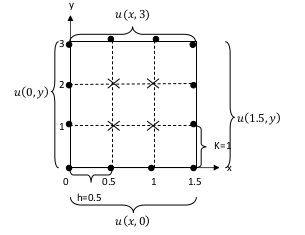
\includegraphics[scale=0.75]{img_Sol_1}
\caption{Mallado de intervalo}
\label{figura3}
\end{center}
\end{figure}
\\Los puntos negros, son los puntos de frontera o en este caso llamados puntos de borde o contorno.\\Las aspas en la malla son las incognitas que tenemos que resolver.\\
Como nuestro problema consta de segundas derivadas parciales, debemos ocupar la que corresponde a este caso, es decir:\\
Para el paso de factor h(relativo al eje X)\\
$$
\frac{\partial^2 u(x_{i},y_{j})}{\partial x^2} \approx \frac{u_{i+1,j}-2u_{i,j}+u_{i-1,j}}{h^2}
$$
Para el paso de factor k(relativo al eje Y)\\
$$
\frac{\partial^2 u(x_{i},y_{j})}{\partial y^2} \approx \frac{u_{i,j+1}-2u_{i,j}+u_{i,j-1}}{k^2}
$$
Reemplazando estos datos en la ecuación diferencial parcial, obtenemos:
$$
\nabla^2 u(x,y) = \frac{\partial^2 u(x,y)}{\partial x^2} + \frac{\partial^2 u(x,y)}{\partial y^2} = 0
$$
$$
\nabla^2 u(x_{i},y_{j}) = \frac{\partial^2 u(x_{i},y_{j})}{\partial x^2} + \frac{\partial^2 u(x_{i},y_{j})}{\partial y^2} \approx \frac{u_{i+1,j}-2u_{i,j}+u_{i-1,j}}{h^2} + \frac{u_{i,j+1}-2u_{i,j}+u_{i,j-1}}{k^2} = 0
$$
Siendo h=0.5 y k=1, se tiene:
$$
4u_{i+1,j}-8u_{i,j}+4u_{i-1,j} + u_{i,j+1}-2u_{i,j}+u_{i,j-1} = 0
$$
$$
4u_{i-1,j} - 10u_{i,j} + u_{i,j+1} + u_{i,j-1} + 4u_{i+1,j}=0
$$
Ahora segun el algoritmo (1) visto anteriormente:\\
Ecuaciones de sistema
se calcula para cada punto las aproximaciones de taylor para i desde 1 hasta 2 y j desde 1 hasta 2, obtenemos:\\
i=1,~~j=1: $$4u_{0,1} - 10u_{1,1} + u_{1,2} + u_{1,0} + 4u_{2,1}=0$$ 
i=1,~~j=2: $$4u_{0,2} - 10u_{1,2} + u_{1,3} + u_{1,1} + 4u_{2,2}=0$$
i=2,~~j=1: $$4u_{1,1} - 10u_{2,1} + u_{2,2} + u_{2,0} + 4u_{3,1}=0$$
i=2~~j=2: $$4u_{1,2} - 10u_{2,2} + u_{2,3} + u_{2,1} + 4u_{3,2}=0$$
Ahora calculamos nuestras condiciones de contorno, las cuales son:\\
$u_{0,1}=u(0,1)=4$\\
$u_{0,2}=u(0,2)=5$\\
$u_{1,0}=u(0.5,0)=1.25$\\
$u_{1,3}=u(0.5,3)=1.5$\\
$u_{2,0}=u(1,0)=2$\\
$u_{3,1}=u(1.5,1)=6$\\
$u_{2,3}=u(1,3)=3$\\
$u_{3,2}=u(1.5,2)=8$\\
Reemplazando estos valores en las ecuaciones de sistema se obtiene:\\
i=1,~~j=1: $$4*4 - 10u_{1,1} + u_{1,2} + 1.25 + 4u_{2,1}=0$$ 
i=1,~~j=2: $$4*5 - 10u_{1,2} + 1.5 + u_{1,1} + 4u_{2,2}=0$$
i=2,~~j=1: $$4u_{1,1} - 10u_{2,1} + u_{2,2} + 2 + 4*6=0$$
i=2~~j=2: $$4u_{1,2} - 10u_{2,2} + 3 + u_{2,1} + 4*8=0$$
Ordenando las ecuaciones:\\
$$- 10u_{1,1} + u_{1,2} + 4u_{2,1} = -17.25$$ 
$$- 10u_{1,2} + u_{1,1} + 4u_{2,2} = -21.5$$
$$4u_{1,1} - 10u_{2,1} + u_{2,2} = -26$$
$$4u_{1,2} - 10u_{2,2} + u_{2,1} = -35$$
Se obtuvo un sistema de ecuaciones lineales de la forma Au=f\\
$$\left\{\begin{array}{crl}
\displaystyle- 10u_{1,1} + u_{1,2} + 4u_{2,1} = -17.25\\
- 10u_{1,2} + u_{1,1} + 4u_{2,2} = -21.5\\
4u_{1,1} - 10u_{2,1} + u_{2,2} = -26\\
4u_{1,2} - 10u_{2,2} + u_{2,1} = -35
\end{array}\right.
$$
Ordenando matricialmente:\\
$$
\left\{\begin{array}{cccc}
    -10 & 1 & 4 & 0 \\
    1 & -10 & 0 & 4 \\
    4 & 0 & -10 & 1 \\
    0 & 4 & 1 & -10 \\
    \end{array}\right\}
\left\{\begin{array}{c}
    u_{1,1}\\
    u_{1,2}\\
    u_{2,1}\\
    u_{2,2}\\
    \end{array}\right\}
    =
\left\{\begin{array}{c}
    -17.25\\
    -21.5\\
    -26\\
    -35\\
    \end{array}\right\}
$$
Ahora usando cualquier tipo de método para resolver sistemas de ecuaciones lineales, en este caso use el método de gauss, se obtiene:\\
$$
\left\{\begin{array}{c}
    u_{1,1}\\
    u_{1,2}\\
    u_{2,1}\\
    u_{2,2}\\
    \end{array}\right\}
=
\left\{\begin{array}{c}
    4.1656\\
    4.9537\\
    4.863\\
    5.9678\\
    \end{array}\right\}
$$
Que son los valores de la Temperatura en los puntos discretos de la placa, como se ve en la figura ~\ref{figura4}
\begin{figure}[htbp]
\begin{center}
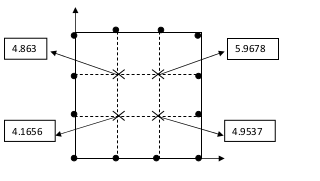
\includegraphics[scale=0.75]{img_Sol_2}
\caption{Mallado de intervalo con todos los puntos}
\label{figura4}
\end{center}
\end{figure}

Usar el programa adjunto llamado metodoAnalitico.m de la siguiente forma:\\
metodoAnalitico(1.5,3,0.5,1,1e-07,30) donde se definen en los apartados f1.m f2.m f3.m y f4.m las funciones de contorno para la ecuacion.\\
Usando meshc(X,Y,U,'LineWidth',2) y view(30,45) se generan las imagenes de la solucion hacemos una grafica para divisar las lineas de contorno en la figura ~\ref{figura5}\\
Para obtener la solucion total, ejecute ecuacionCalorEstacionarioNumerico.m, y obtendrá todo el resultado.
\begin{figure}[htbp]
\begin{center}
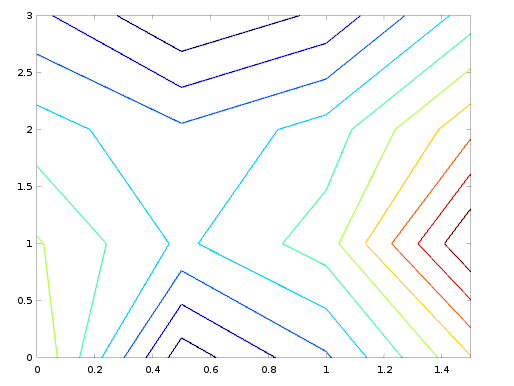
\includegraphics[scale=0.75]{img_Sol_4}
\caption{Lineas de contorno de la solucion analítica}
\label{figura5}
\end{center}
\end{figure}
\\Y a su vez se muestra la grafica de superficie de la solucion numerica en la figura ~\ref{figura6}
\begin{figure}[htbp]
\begin{center}
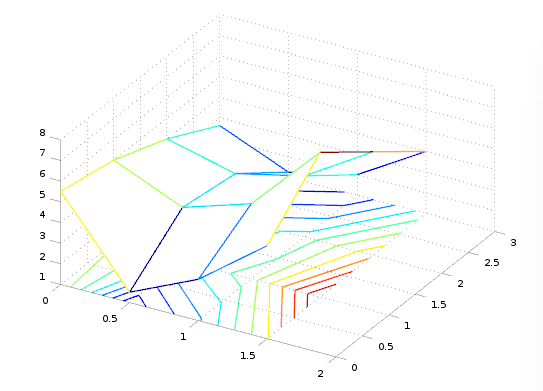
\includegraphics[scale=0.65]{img_Sol_3}
\caption{Superficie solución numérica de la ecuación de calor estacionaria}
\label{figura6}
\end{center}
\end{figure}

\subsection{Solución Análitica}
\thispagestyle{empty}
Para esta seccion se analizara la solución de el siguiente problema:\\
Se tomara que entra a equilibrio térmico desde t=0.\\
$$
\nabla^2 u(x,y)=\frac{\partial^2 u(x,y)}{\partial x^2} + \frac{\partial^2 u(x,y)}{\partial y^2} = 0
$$
Donde: $$ u:\Omega \subseteq \left[0,1.5\right]X\left[0,3\right] \rightarrow \Re$$
Con condiciones:\\
u(0,y)=y + 3,~~~  u(1.5,y)=2y + 4,~~~  $u(x,0) = x^2 + 1 $,~~~  u(x,3) = 3x.\\
donde $ 0 \le x \le 1.5 $ y $ 0 \le y \le 3 $\\
Se ve que es una ecuación diferencial parcial de Laplace, elíptica y homogénea.\\
Haciendo el artificio que u(x,y)=T(x,y)=X(x) Y(y),\\ 
Tenemos que:\\
$\frac{\partial^2 T(x,y)}{\partial x^2} = X''(x)Y(y)$ y $\frac{\partial^2 T(x,y)}{\partial y^2} = X(x)Y''(y)$\\
Reemplazamos:\\
$ X''(x)Y(y) + X(x)Y''(y) = 0$, dividiendo entre X(x)Y(y) obtenemos:\\
$ \frac{X''(x)}{X(x)} + \frac{Y''(y)}{Y(y)} = 0$
Hacemos $ X''(x) = - n^2 X(x) $ y $ Y''(y) =  n^2 Y(y) $\\
de tal manera que se forme:
$ X''(x) + n^2 X(x) =0$ y $ Y''(y) -  n^2 Y(y)=0 $, entonces como $n^2 \ge 0 $\\
La solución de X y Y vienen dados de la forma:\\
$ X(x) = C_1 \cos(nx)+C_2 \sin(nx)  $ \\
y\\
$ Y(y) = C_3 \cosh(ny)+C_4 \sinh(ny) $ \\
Reemplazamos en T(x,y)=X(x)Y(y), T(x,y)=$\left( C_1 \cos(nx)+C_2 \sin(nx)\right) \left(C_3 \cosh(ny)+C_4 \sinh(ny)\right) $\\
Tenemos que:\\
para x=0 y para todo y, T(0,y)=y+3 = $C_1\left( C_3 \cosh(ny)+C_4 \sinh(ny)\right) $\\
para x=1.5 y para todo y, T(1.5,y)=2y+4 = $\left( C_1 \cos(1.5n)+C_2 \sin(1.5n)\right) \left( C_3 \cosh(ny)+C_4 \sinh(ny)\right) $\\
para y=0 y para todo x, T(x,0)=$x^2 + 1 $ = $\left( C_1 \cos(nx)+C_2 \sin(nx)\right)( C_3)  $\\
para y=3 y para todo x, T(x,3)=3x=$\left( C_1 \cos(nx)+C_2 \sin(nx)\right) \left(C_3 \cosh(3n)+C_4 \sinh(3n)\right) $\\
Derivando:\\
1=$C_1\left( nC_3 \sinh(ny)+nC_4 \cosh(ny)\right) $...(1)\\
2=$\left( C_1 \cos(1.5n)+C_2 \sin(1.5n)\right)\left( nC_3 \sinh(ny)+nC_4 \cosh(ny)\right) $...(2)\\
2x = $\left(- nC_1 \sin(nx)+ nC_2 \cos(nx)\right)( C_3)  $...(3)\\
3=$\left(- nC_1 \sin(nx)+ nC_2 \cos(nx)\right) \left(C_3 \cosh(3n)+C_4 \sinh(3n)\right) $...(4)\\
De las ecuaciones (1) y (2) obtenemos:\\
$C_2 = C_1 \left( 2\csc(1.5n) - \cot(1.5n)\right)$\\
De las ecuaciones (3) y (4) obtenemos:\\
$C_4 = C_3 \left( \frac{3-2x\cosh(3n)}{2x\sinh(3n)}\right)$, entonces $C_4$ depende de x.\\Volviendo a T(x,y)=X(x)Y(y).\\
T(x,y)=$C_1C_3\left( \cos(nx)+ \left(2\csc(1.5n) - \cot(1.5n)\right) \sin(nx)\right) \left(\cosh(ny)+\left( \frac{3-2x\cosh(3n)}{2x\sinh(3n)}\right) \sinh(ny)\right) $\\
Evaluando para x=1.5 y y=0.\\
T(1.5,0)=~4~=$C_1C_3\left( \cos(1.5n)+ \left(2\csc(1.5n) - \cot(1.5n)\right) \sin(1.5n)\right) \left(\cosh(0)+\left( \frac{3-3\cosh(3n)}{3\sinh(3n)}\right) \sinh(0)\right) $\\T(1.5,0) =~4~= $ C_1C_3\left( \cos(1.5n)+ \left(2 - \cos(1.5n)\right)\right) \left(\cosh(0)\right) $ = $ 2C_1C_3 $ \\Entonces $C_1 C_3 = 2$\\
Ahora falta el valor o posibles valores de n.\\
Evaluando para x=0 y y=3.\\
T(0,3) = ~0~=$ C_1 \left(C_3 \cosh(3n)+C_4 \sinh(3n)\right) $\\
Haciendo n=$m\pi$, donde m es entero, la ecuación queda así:\\
T(0,3) = ~0~=$ C_1 \left(C_3 \cosh(3m\pi)+C_4 \sinh(3m \pi)\right) $\\
T(0,3) = ~0~=$ C_1 C_3 \cosh(3m\pi)+C_1 C_4 \sinh(3m \pi) $\\
De lo anterior:\\
T(0,3) = ~0~=$ 2 \cosh(3m\pi)+C_1 C_4 \sinh(3m \pi) $\\
n=$\frac{1}{\pi}$\\
Por lo tanto la solución analítica es:\\
$$T(x,y)=2\left( \cos(\frac{x}{\pi})+ \left(2\csc(\frac{3}{2\pi}) - \cot(\frac{3}{2\pi})\right) \sin(\frac{x}{\pi})\right) \left(\cosh(\frac{y}{\pi})+\left( \frac{3-2x\cosh(\frac{3}{\pi})}{2x\sinh(\frac{3}{\pi})}\right) \sinh(\frac{y}{\pi})\right) $$\\
Graficando la función en el dominio de $[0,1.5]X[0,3]$ tenemos mediante el programa metodoAnalitico.m que devuelve las siguientes graficas de solucion.
se muestrasn las lineas de contorno en la figura
~\ref{figura7} y en la figura ~\ref{figura8} se muestran la superficie solución.
\begin{figure}[htbp]
\begin{center}
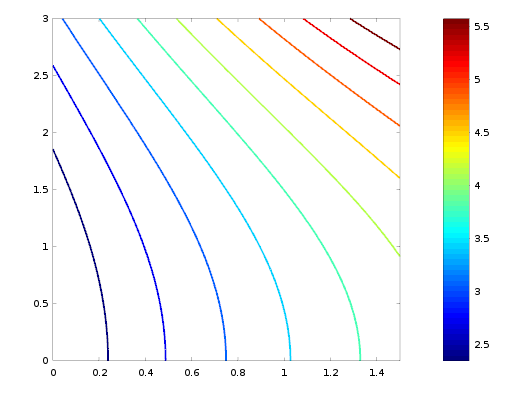
\includegraphics[scale=0.65]{img_Sol_5}
\caption{Lineas de contorno de la solución analítica}
\label{figura7}
\end{center}
\end{figure}

\begin{figure}[htbp]
\begin{center}
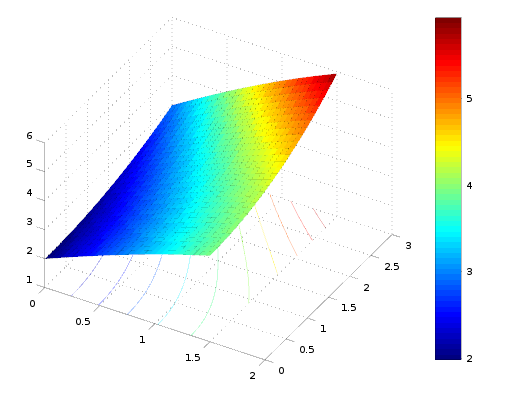
\includegraphics[scale=0.65]{img_Sol_6}
\caption{Superficie solución analítica de la ecuación de calor estacionaria}
\label{figura8}
\end{center}
\end{figure}

\newpage
\section{Conclusiones}
Haciendo la comparación entre la solución analítica y la numérica, se observa que sus valores no difieren por mucho salvo un error de $10^{-04}$. por lo que esta solución en diferencias finitas, es un buen modelo numérico a utilizar en ecuaciones elípticas estacionarias.
\section{Referencias}
Springer, Partial Differential Equations With Numerical Methods - 2009.
\end{document}
